%----------------------------------------------------------------------------------------
%	PACKAGES AND DOCUMENT CONFIGURATIONS
%----------------------------------------------------------------------------------------

\documentclass[10pt,a4paper]{article}

\usepackage[utf8]{inputenc}
\usepackage[spanish]{babel}
\usepackage{siunitx} % Provides the \SI{}{} and \si{} command for typesetting SI units
\usepackage{graphicx} % Required for the inclusion of images
\graphicspath{ {images/} }
\usepackage{natbib} % Required to change bibliography style to APA
\usepackage{amsmath, amsfonts, amssymb} % Required for some math elements 
\usepackage{booktabs} %\toprule and tablas
\usepackage{hyperref}
\usepackage{rotating}
\usepackage{enumitem}
\usepackage{float}
\usepackage{colortbl}
\usepackage[margin=0.7in]{geometry}
\usepackage{cancel}
\usepackage{lipsum}% http://ctan.org/pkg/lipsum
\usepackage{fancyhdr}% http://ctan.org/pkg/fancyhdr
\usepackage{multirow}
\usepackage[table,xcdraw]{xcolor}
%\setlength\parindent{0pt} % Removes all indentation from paragraphs
\renewcommand{\labelenumi}{\alph{enumi}.} % Make numbering in the enumerate environment by letter rather than number (e.g. section 6)

\usepackage{times} % Uncomment to use the Times New Roman font

\usepackage{authblk} % author package
\renewcommand*{\Authand}{, } % para separar los autores por comas

\newcolumntype{P}[1]{>{\centering\arraybackslash}p{#1}}
\newcolumntype{M}[1]{>{\centering\arraybackslash}m{#1}}

\usepackage{makecell}%To keep spacing of text in tables
\setcellgapes{4pt}%parameter for the spacing


% to use tables visit http://www.tablesgenerator.com/latex_tables
\usepackage{multirow} % para usar multiples filas en una tabla

\setlength{\parindent}{0cm}
\def\thesubsection{\roman{subsection}}
\def\thesubsubsection{\alph{subsubsection}}

\newcommand\NP{97490}

%----------------------------------------------------------------------------------------
%	DOCUMENT INFORMATION
%----------------------------------------------------------------------------------------

\title{%
  Análisis Numérico - TP 1 \\
  \large Ecuaciones no lineales en sistemas mecánicos}

\author{Rocío Gallo, padrón 97490 (rochimgg@gmail.com)\\ Facundo Monpelat, padrón 92716 (facundo.monpelat@gmail.com)}

\date{\today} %Date for the report


\begin{document}
%\begin{centering}
%\begin{align*}
% &Rocío Gallo, &&padrón 97490 &&(rochimgg@gmail.com)\\
 %&Facundo Monpelat, &&padrón 92716 &&(facundo.monpelat@gmail.com)
%\end{align*}


\maketitle % Insert the title, author and date

\section{Introducción}

El siguiente trabajo práctico consiste en la resolución de un sistema mecánico de dos resortes de longitud natural $L_{0}$ unidos a una masa puntual de valor $m$. La distancia entre el extremo fijo de cada resorte y el eje vertical por el cual pasa la masa será de valor $a$.\\

El número de padrón utilizado para efectuar el calculo de $L_{o}$ será el de Rocío Gallo (97490). Para efectuar los cálculos, se redondearán los datos a tres decimales.\\

\definecolor{Gray}{gray}{0.85}

\section{Objetivos}
\begin{enumerate}
\item Experimentar con el uso de métodos numéricos la resolución de ecuaciones no lineales.
\item Integrar conocimientos de mecánica.
\end{enumerate}

\section{Desarrollo}

Los valores de los parámetros contemplando el padrón serán los siguientes:
\begin{table}[h]
\centering 
\begin{tabular}{|>{\columncolor[HTML]{EFEFEF}}l |l|l|}
\hline
\multicolumn{1}{|c|}{\cellcolor[HTML]{EFEFEF}}                                                                                        & L$_{0}$ {[}m{]} & 2,052 \\ \cline{2-3} 
\multicolumn{1}{|c|}{\multirow{-2}{*}{\cellcolor[HTML]{EFEFEF}\begin{tabular}[c]{@{}c@{}}Propiedades de los\\ resortes\end{tabular}}} & k{[}N/m{]}       & 10     \\ \hline
Masa de referencia                                                                                                                    & m$_{0}$        & 1,026 \\ \hline
Geometría                                                                                                                             & a{[}m{]}         & 1      \\ \hline
\end{tabular}
\end{table}    


\subsection{Ejercicio 1}
 El objetivo es encontrar los puntos de equilibrio del sistema sin tener en cuenta el efecto de la gravedad. Como en un punto de equilibrio $F_{Res} = 0$ y con $m=0$, se puede despejar fácilmente la variable $y$, y dejarla en función de las demás incógnitas.\\

Caso inicial

\begin{equation}
\begin{split}
\notag F_{\text{Res}}(y)=-2Ky\left(1-\frac{L_{\text{0}}}{\sqrt{Y^2+a^2}}\right)-mg
\end{split}
\end{equation}

Como $a<L_{0}$ nos encontramos en el caso en el cual el sistema tiene tres puntos de equilibrio: Dos estables y uno inestable en el eje horizontal, del cual están fijados los resortes.\\[20pt]

Despejando $y$ de la ecuación de fuerza\\

\begin{centering}
$\left\{
\begin{array}{rcl}
      &y_{1}&=0     \hspace{53pt} Equilibrio\;inestable\\[7pt]
      &y_{2}&=\sqrt{L_{0}^{2}-a^{2}}  \hspace{15pt}    \underline{Equilibrio\;estable}\\[7pt]
      &y_{3}&= -\sqrt{L_{0}^{2}-a^{2}}  \hspace{8pt}   Equilibrio\;estable\\
\end{array}\right. $\\[10pt]
\end{centering}

Analizaremos el caso de la raíz positiva de la ecuación de $F_{Res}$ con los métodos numéricos de Bisección, Punto fijo y Newton-Raphson.

Como para el caso particular $m=0$, los puntos de equilibrio fueron encontrados de manera analítica, se puede calcular el error de truncamiento de $y(L_{0},a)$

Por teoría de dispersión de errores
\begin{equation}
\notag \Delta(y)= \left|\dfrac{\partial y}{\partial L_{0}}\right| \Delta(L_{0})+ \left|\dfrac{\partial y}{\partial a}\right| \Delta(a)
\end{equation}

Suponiendo que $a$ no tiene error, por ser dato del enunciado 

\begin{equation}
\notag \Delta(y)= \left|\dfrac{\partial y}{\partial L_{0}}\right| \Delta(L_{0}) =\left|\dfrac{\partial}{\partial L_{0}} \left(\sqrt{L_{0}^{2}-a^{2}}\right)\right|\Delta(L_{0})=\left| \dfrac{\bcancel{2}L_{0}}{\bcancel{2}\sqrt{L_{0}^{2}-a^{2}}} \right|
\end{equation}

Remplazando con los datos

\begin{equation}
\notag \Delta (y)=\left|\dfrac{2,052}{\sqrt{2,052^{2}+1^{2}}}\right|0,001=0,001145...\;m\Rightarrow \text{Error debido al redondeo de } L_{0}
\end{equation}
\\

Por métodos numéricos, la raíz positiva hallada con una diferencia relativa menor a $0.5 10^{-15}$ por cada método fue:

\begin{itemize}
\item Bisección: $1.790698467079256 \pm 0.5\:10^{-15}$ con 52 iteraciones.
\item Punto Fijo: $1.790698467079257 \pm 0.5\:10^{-15}$ Con  27 iteraciones.
\item Newton-Raphson: $1.790698467079257 \pm 0.5\:10^{-15}$ con 7 iteraciones.
\end{itemize}

~\\ % vertical mode break same as: \leavevmode
\newline
\newline


\subsubsection{Tabla referente a Bisección}

\begin{table}[H]
\makegapedcells
\centering
%{Método de Bisección.\label{clist}}
\resizebox{0.55\textwidth}{!}{
\begin{tabular}{|c|c|c|c|c|c|c|c|}
\hline k & a$_{k}$ & b$_{k}$ & f(a$_{k}$) & f(b$_{k}$) & r$_{k+1}$ & $\Delta r_{k+1}$ & $\dfrac{\Delta r}{r}$ \\
\hline 1 & 1.6000 & 3.0000 & 2.7849 & -21.0850 & 2.2999999999999998 & 0.7000 & 0.3043 \\
\hline 2 & 1.6000 & 2.3000 & 2.7849 & -8.3818 & 1.9499999999999997 & 0.3500 & 0.1795 \\
\hline 3 & 1.6000 & 1.9500 & 2.7849 & -2.4997 & 1.7749999999999999 & 0.1750 & 0.0986 \\
\hline 4 & 1.7750 & 1.9500 & 0.2386 & -2.4997 & 1.8624999999999998 & 0.0875 & 0.0470 \\
\hline 5 & 1.7750 & 1.8625 & 0.2386 & -1.1097 & 1.8187499999999999 & 0.0437 & 0.0241 \\
\hline 6 & 1.7750 & 1.8187 & 0.2386 & -0.4300 & 1.7968750000000000 & 0.0219 & 0.0122 \\
\hline 7 & 1.7750 & 1.7969 & 0.2386 & -0.0943 & 1.7859375000000000 & 0.0109 & 0.0061 \\
\hline 8 & 1.7859 & 1.7969 & 0.0725 & -0.0943 & 1.7914062500000001 & 0.0055 & 0.0031 \\
\hline 9 & 1.7859 & 1.7914 & 0.0725 & -0.0108 & 1.7886718749999999 & 0.0027 & 0.0015 \\
\hline 10 & 1.7887 & 1.7914 & 0.0309 & -0.0108 & 1.7900390625000000 & 0.0014 & 0.0008 \\
\hline 43 & 1.7907 & 1.7907 & 0.0000 & -0.0000 & 1.7906984670793233 & 0.0000 & 0.0000 \\
\hline 44 & 1.7907 & 1.7907 & 0.0000 & -0.0000 & 1.7906984670792436 & 0.0000 & 0.0000 \\
\hline 45 & 1.7907 & 1.7907 & 0.0000 & -0.0000 & 1.7906984670792836 & 0.0000 & 0.0000 \\
\hline 46 & 1.7907 & 1.7907 & 0.0000 & -0.0000 & 1.7906984670792636 & 0.0000 & 0.0000 \\
\hline 47 & 1.7907 & 1.7907 & 0.0000 & -0.0000 & 1.7906984670792536 & 0.0000 & 0.0000 \\
\hline 48 & 1.7907 & 1.7907 & 0.0000 & -0.0000 & 1.7906984670792587 & 0.0000 & 0.0000 \\
\hline 49 & 1.7907 & 1.7907 & 0.0000 & -0.0000 & 1.7906984670792561 & 0.0000 & 0.0000 \\
\hline 50 & 1.7907 & 1.7907 & 0.0000 & -0.0000 & 1.7906984670792574 & 0.0000 & 0.0000 \\
\hline 51 & 1.7907 & 1.7907 & 0.0000 & -0.0000 & 1.7906984670792567 & 0.0000 & 0.0000 \\
\hline 52 & 1.7907 & 1.7907 & 0.0000 & -0.0000 & 1.7906984670792565 & 0.0000 & 0.0000 \\
\hline
\end{tabular}}
\caption{Bisección Intervalo: [0,2;3].}
\end{table}
Raíz: 1.7906984670792565 $\pm 0.5\:10^{-15}$


~\\ % vertical mode break same as: \leavevmode
~\\ 

\subsubsection{Tabla referente a Punto Fijo}

\begin{table}[H]
\makegapedcells
\centering
\resizebox{0.35\textwidth}{!}{
\begin{tabular}{|c|c|c|c|c|c|}
\hline k & Y$_{k}$ & $\Delta$ Y & $\dfrac{\Delta Y}{Y_{k}}$ \\
\hline 1 & 1.198408992708251 & 0.4784 & 0.3992 \\
\hline 2 & 1.574764682354527 & 0.3764 & 0.2390 \\
\hline 3 & 1.731406147305723 & 0.1566 & 0.0905 \\
\hline 4 & 1.776052759159591 & 0.0446 & 0.0251 \\
\hline 5 & 1.787184055449170 & 0.0111 & 0.0062 \\
\hline 6 & 1.789861137197377 & 0.0027 & 0.0015 \\
\hline 7 & 1.790499309192340 & 0.0006 & 0.0004 \\
\hline 8 & 1.790651116922637 & 0.0002 & 0.0001 \\
\hline 9 & 1.790687210583034 & 0.0000 & 0.0000 \\
\hline 10 & 1.790695791147518 & 0.0000 & 0.0000 \\
\hline 18 & 1.790698467051965 & 0.0000 & 0.0000 \\
\hline 19 & 1.790698467072769 & 0.0000 & 0.0000 \\
\hline 20 & 1.790698467077715 & 0.0000 & 0.0000 \\
\hline 21 & 1.790698467078891 & 0.0000 & 0.0000 \\
\hline 22 & 1.790698467079170 & 0.0000 & 0.0000 \\
\hline 23 & 1.790698467079236 & 0.0000 & 0.0000 \\
\hline 24 & 1.790698467079252 & 0.0000 & 0.0000 \\
\hline 25 & 1.790698467079256 & 0.0000 & 0.0000 \\
\hline 26 & 1.790698467079257 & 0.0000 & 0.0000 \\
\hline 27 & 1.790698467079257 & 0.0000 & 0.0000 \\
\hline
\end{tabular}}
\caption{Punto fijo Semilla: 0,72}
\end{table}
Raíz: 1.790698467079257 $\pm 0.5\:10^{-15}$

\subsubsection{Tabla referente a Newton-Raphson}

\begin{table}[H]
\makegapedcells
\centering
\resizebox{0.35\textwidth}{!}{
\begin{tabular}{|c|c|c|c|c|c|}
\hline k & Y$_{k}$ & $\Delta$ Y & $\dfrac{\Delta Y}{Y_{k}}$ \\
\hline 1 & 2.638189400285716 & 1.6382 & 0.6210 \\
\hline 2 & 1.845449360471512 & 0.7927 & 0.4296 \\
\hline 3 & 1.791250851256665 & 0.0542 & 0.0303 \\
\hline 4 & 1.790698527791094 & 0.0006 & 0.0003 \\
\hline 5 & 1.790698467079258 & 0.0000 & 0.0000 \\
\hline 6 & 1.790698467079257 & 0.0000 & 0.0000 \\
\hline 7 & 1.790698467079257 & 0.0000 & 0.0000 \\
\hline
\end{tabular}}
\caption{Newton-Raphson Semilla: 1}
\end{table}

Raíz: $1.790698467079257 \pm 0.5\:10^{-15}$.
\\
\\
Gráfica de la diferencia absoluta entre dos iteraciones para cada método, con escala logarítmica en el eje Y y cantidad de iteraciones en el eje X para apreciar correctamente los órdenes de magnitud de cada uno de los procedimientos.

\begin{figure}[H]
\centering
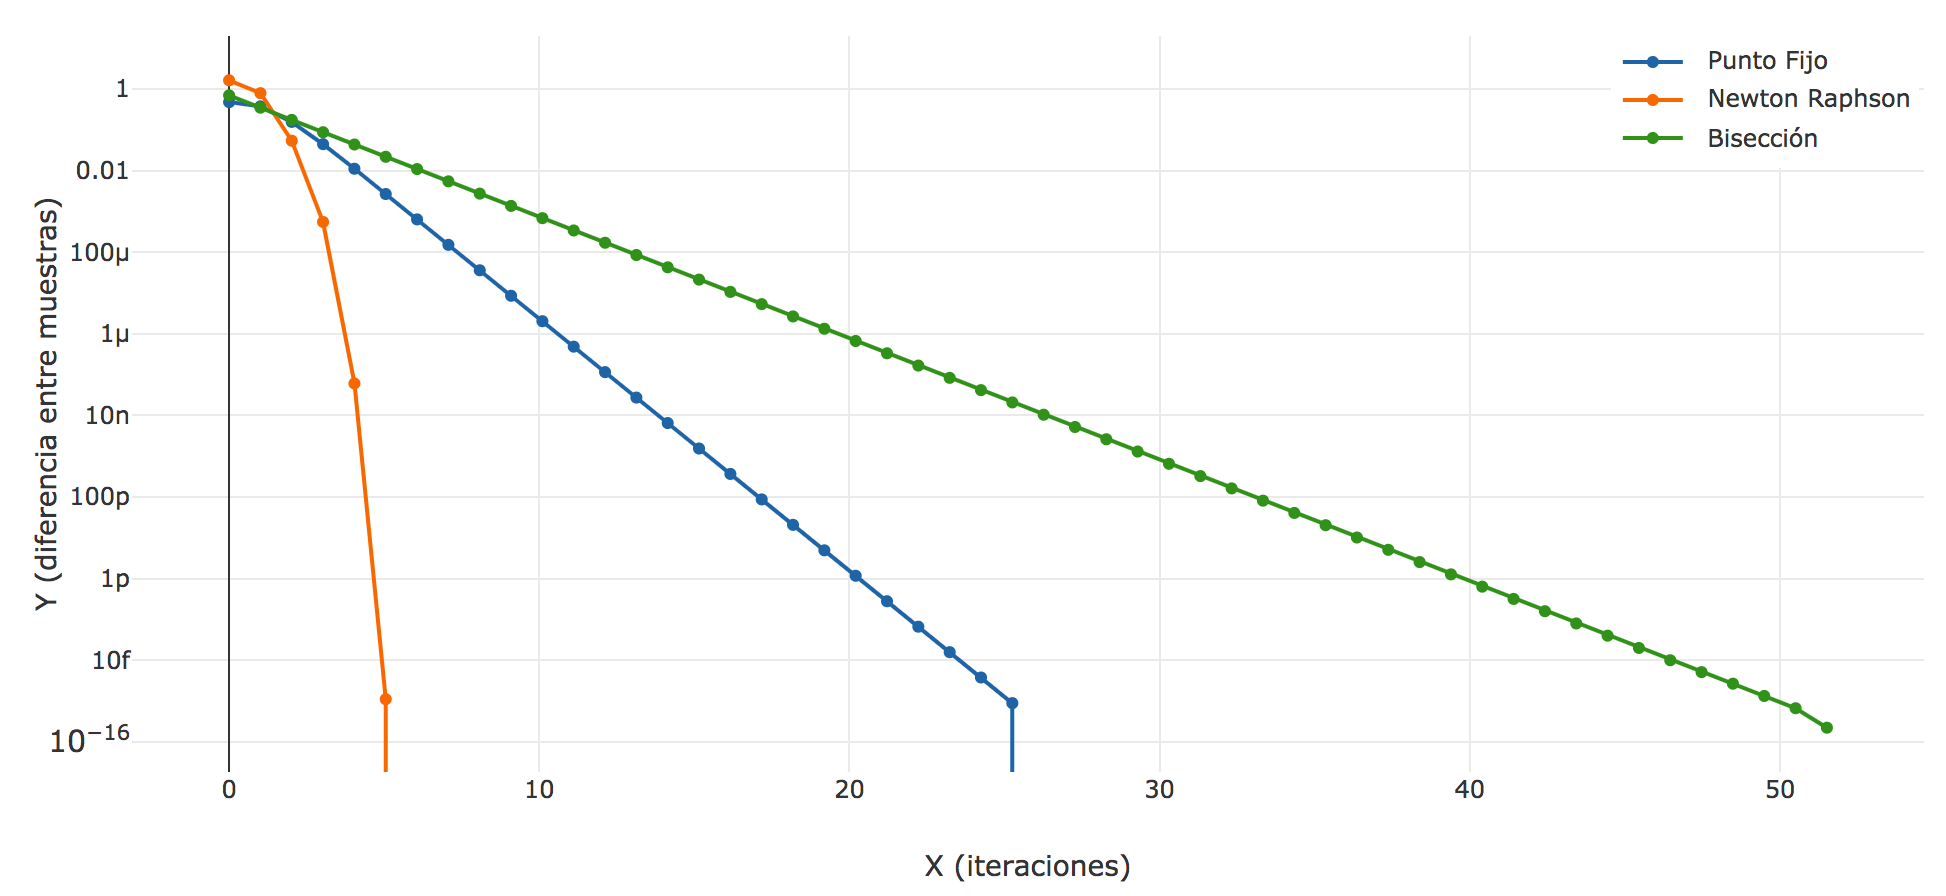
\includegraphics[width=15cm]{ej1.png}
\caption{Convergencias de cada método.}
\end{figure}

% ------------------------
\subsection{Ejercicio 2}
% ------------------------
 Para el caso de $m=0.3*m_{0}$ no es tan sencillo encontrar los puntos de equilibrio como para el caso de masa despreciable, por lo que las raíces serán halladas mediante métodos numéricos.\\

Como estamos en el mismo caso en que $a<L_{0}$ encontraremos tres puntos de equilibrio.

Como todas las fuerzas que interactúan en el sistema son conservativas, podemos usar la relación:

\begin{equation}
    \notag-\dfrac{dE_{Pot}}{dy}= \sum{F_{Cons}(y)}
\end{equation}
\\

Para este caso, supondremos que la partícula solo tiene movimiento en el eje y. Calculamos las fuerzas (se toma positivo hacia abajo y el cero en el eje horizontal a los extremos fijos de cada resorte).

\begin{equation}
\notag \sum{F_{y}}=mg-2F_{Elas}\cos{(\theta)}
\end{equation}

A partir de estas fuerzas hallaremos la energía potencial en el eje $y$ $E_{Pot}$.
\\

\begin{equation}
\notag E_{Pot} = mgy-\dfrac{\bcancel{2}}{\bcancel{2}}K(\Delta y)^{2}=mgy-K(\Delta y)^{2}
\end{equation}
\\

Observar que $\Delta y$ es el estiramiento en el eje $y$ y no el error de dispersión, como había sido en el ejercicio 1. Para fines prácticos, en este sistema $\Delta y=L_{Eq}-L_{0}$ ($L_{Eq}=\sqrt{y^{2}+a^{2}}$ es la nueva longitud natural del resorte, debido a la masa $m$).

\begin{equation}
\notag E_{Pot}=-mgy+k[(L_{Eq}-L_{0})\cos{(\theta)}]^{2}
\end{equation}


Para hallar $\sum{F_{Cons}}$, se deriva la expresión de la energía potencial.
\\

\begin{equation}
\notag \sum{F_{Cons}}=F_{Res}=mg-2Ky=0.3m_{0}g-2k(L_{Eq}-L_{0})
\end{equation}

Esta expresión puede ser usada para corroborar resultados más adelante.\\

\subsubsection{Raíces por el método Bisección.}
Tomando el intervalo [-3;-1], se encuentra por este método la raíz negativa -1.9819518625863082 $\pm 0.5\:10^{-15}$.

\begin{table}[H]
\makegapedcells
\centering
\resizebox{0.55\textwidth}{!}{
\begin{tabular}{|c|c|c|c|c|c|c|c|}
\hline k & a$_{k}$ & b$_{k}$ & f(a$_{k}$) & f(b$_{k}$) & r$_{k+1}$ & $\Delta r_{k+1}$ & $\dfrac{\Delta r}{r}$ \\
\hline 1 & -2.0000 & -1.0000 & 0.2940 & -12.0221 & -1.5000000000000000 & 0.5000 & -0.3333 \\
\hline 2 & -2.0000 & -1.5000 & 0.2940 & -7.1473 & -1.7500000000000000 & 0.2500 & -0.1429 \\
\hline 3 & -2.0000 & -1.7500 & 0.2940 & -3.6319 & -1.8750000000000000 & 0.1250 & -0.0667 \\
\hline 4 & -2.0000 & -1.8750 & 0.2940 & -1.7107 & -1.9375000000000000 & 0.0625 & -0.0323 \\
\hline 5 & -2.0000 & -1.9375 & 0.2940 & -0.7178 & -1.9687500000000000 & 0.0312 & -0.0159 \\
\hline 6 & -2.0000 & -1.9688 & 0.2940 & -0.2141 & -1.9843750000000000 & 0.0156 & -0.0079 \\
\hline 7 & -1.9844 & -1.9688 & 0.0394 & -0.2141 & -1.9765625000000000 & 0.0078 & -0.0040 \\
\hline 8 & -1.9844 & -1.9766 & 0.0394 & -0.0875 & -1.9804687500000000 & 0.0039 & -0.0020 \\
\hline 9 & -1.9844 & -1.9805 & 0.0394 & -0.0241 & -1.9824218750000000 & 0.0020 & -0.0010 \\
\hline 10 & -1.9824 & -1.9805 & 0.0076 & -0.0241 & -1.9814453125000000 & 0.0010 & -0.0005 \\
\hline 42 & -1.9820 & -1.9820 & 0.0000 & -0.0000 & -1.9819518625861292 & 0.0000 & -0.0000 \\
\hline 43 & -1.9820 & -1.9820 & 0.0000 & -0.0000 & -1.9819518625862429 & 0.0000 & -0.0000 \\
\hline 44 & -1.9820 & -1.9820 & 0.0000 & -0.0000 & -1.9819518625862997 & 0.0000 & -0.0000 \\
\hline 45 & -1.9820 & -1.9820 & 0.0000 & -0.0000 & -1.9819518625863282 & 0.0000 & -0.0000 \\
\hline 46 & -1.9820 & -1.9820 & 0.0000 & -0.0000 & -1.9819518625863140 & 0.0000 & -0.0000 \\
\hline 47 & -1.9820 & -1.9820 & 0.0000 & -0.0000 & -1.9819518625863068 & 0.0000 & -0.0000 \\
\hline 48 & -1.9820 & -1.9820 & 0.0000 & -0.0000 & -1.9819518625863104 & 0.0000 & -0.0000 \\
\hline 49 & -1.9820 & -1.9820 & 0.0000 & -0.0000 & -1.9819518625863086 & 0.0000 & -0.0000 \\
\hline 50 & -1.9820 & -1.9820 & 0.0000 & -0.0000 & -1.9819518625863077 & 0.0000 & -0.0000 \\
\hline 51 & -1.9820 & -1.9820 & 0.0000 & -0.0000 & -1.9819518625863082 & 0.0000 & -0.0000 \\
\hline
\end{tabular}}
\caption{Bisección intervalo: [-3;-1]}
\end{table}


Tomando el intervalo $[-0,5;0,6]$, se encuentra la primer raíz positiva $0.1465310699476753 \pm 0.5\:10^{-15}$.

\begin{table}[H]
\makegapedcells
\centering
\resizebox{0.55\textwidth}{!}{
\begin{tabular}{|c|c|c|c|c|c|c|c|}
\hline k & a$_{k}$ & b$_{k}$ & f(a$_{k}$) & f(b$_{k}$) & r$_{k+1}$ & $\Delta r_{k+1}$ & $\dfrac{\Delta r}{r}$ \\
\hline 1 & 0.0500 & 0.6000 & -1.9681 & 6.0880 & 0.3250000000000000 & 0.2750 & 0.8462 \\
\hline 2 & 0.0500 & 0.3250 & -1.9681 & 3.1621 & 0.1875000000000000 & 0.1375 & 0.7333 \\
\hline 3 & 0.0500 & 0.1875 & -1.9681 & 0.7929 & 0.1187500000000000 & 0.0687 & 0.5789 \\
\hline 4 & 0.1188 & 0.1875 & -0.5544 & 0.7929 & 0.1531250000000000 & 0.0344 & 0.2245 \\
\hline 5 & 0.1188 & 0.1531 & -0.5544 & 0.1297 & 0.1359375000000000 & 0.0172 & 0.1264 \\
\hline 6 & 0.1359 & 0.1531 & -0.2100 & 0.1297 & 0.1445312500000001 & 0.0086 & 0.0595 \\
\hline 7 & 0.1445 & 0.1531 & -0.0395 & 0.1297 & 0.1488281250000000 & 0.0043 & 0.0289 \\
\hline 8 & 0.1445 & 0.1488 & -0.0395 & 0.0453 & 0.1466796875000000 & 0.0021 & 0.0146 \\
\hline 9 & 0.1445 & 0.1467 & -0.0395 & 0.0029 & 0.1456054687500000 & 0.0011 & 0.0074 \\
\hline 10 & 0.1456 & 0.1467 & -0.0183 & 0.0029 & 0.1461425781250000 & 0.0005 & 0.0037 \\
\hline 41 & 0.1465 & 0.1465 & -0.0000 & 0.0000 & 0.1465310699478096 & 0.0000 & 0.0000 \\
\hline 42 & 0.1465 & 0.1465 & -0.0000 & 0.0000 & 0.1465310699476846 & 0.0000 & 0.0000 \\
\hline 43 & 0.1465 & 0.1465 & -0.0000 & 0.0000 & 0.1465310699476220 & 0.0000 & 0.0000 \\
\hline 44 & 0.1465 & 0.1465 & -0.0000 & 0.0000 & 0.1465310699476533 & 0.0000 & 0.0000 \\
\hline 45 & 0.1465 & 0.1465 & -0.0000 & 0.0000 & 0.1465310699476689 & 0.0000 & 0.0000 \\
\hline 46 & 0.1465 & 0.1465 & -0.0000 & 0.0000 & 0.1465310699476767 & 0.0000 & 0.0000 \\
\hline 47 & 0.1465 & 0.1465 & -0.0000 & 0.0000 & 0.1465310699476728 & 0.0000 & 0.0000 \\
\hline 48 & 0.1465 & 0.1465 & -0.0000 & 0.0000 & 0.1465310699476748 & 0.0000 & 0.0000 \\
\hline 49 & 0.1465 & 0.1465 & -0.0000 & 0.0000 & 0.1465310699476758 & 0.0000 & 0.0000 \\
\hline 50 & 0.1465 & 0.1465 & -0.0000 & 0.0000 & 0.1465310699476753 & 0.0000 & 0.0000 \\
\hline
\end{tabular}}
\caption{Bisección Intervalo: [-0,5;0,6]}
\end{table}

Tomando el intervalo [-0,8;5], se encuentra la segunda raíz positiva 1.5832397676915879 $\pm 0.5\:10^{-15}$.

\begin{table}[H]
\makegapedcells
\centering
\resizebox{0.55\textwidth}{!}{
\begin{tabular}{|c|c|c|c|c|c|c|c|}
\hline k & a$_{k}$ & b$_{k}$ & f(a$_{k}$) & f(b$_{k}$) & r$_{k+1}$ & $\Delta r_{k+1}$ & $\dfrac{\Delta r}{r}$ \\
\hline 1 & 0.8000 & 2.9000 & 6.6084 & -22.2374 & 1.8500000000000003 & 1.0500 & 0.5676 \\
\hline 2 & 0.8000 & 1.8500 & 6.6084 & -3.9310 & 1.3250000000000002 & 0.5250 & 0.3962 \\
\hline 3 & 1.3250 & 1.8500 & 3.2251 & -3.9310 & 1.5875000000000004 & 0.2625 & 0.1654 \\
\hline 4 & 1.3250 & 1.5875 & 3.2251 & -0.0587 & 1.4562500000000003 & 0.1313 & 0.0901 \\
\hline 5 & 1.4563 & 1.5875 & 1.6733 & -0.0587 & 1.5218750000000003 & 0.0656 & 0.0431 \\
\hline 6 & 1.5219 & 1.5875 & 0.8275 & -0.0587 & 1.5546875000000004 & 0.0328 & 0.0211 \\
\hline 7 & 1.5547 & 1.5875 & 0.3892 & -0.0587 & 1.5710937500000004 & 0.0164 & 0.0104 \\
\hline 8 & 1.5711 & 1.5875 & 0.1664 & -0.0587 & 1.5792968750000003 & 0.0082 & 0.0052 \\
\hline 9 & 1.5793 & 1.5875 & 0.0542 & -0.0587 & 1.5833984375000003 & 0.0041 & 0.0026 \\
\hline 10 & 1.5793 & 1.5834 & 0.0542 & -0.0022 & 1.5813476562500002 & 0.0021 & 0.0013 \\
\hline 43 & 1.5832 & 1.5832 & 0.0000 & -0.0000 & 1.5832397676914869 & 0.0000 & 0.0000 \\
\hline 44 & 1.5832 & 1.5832 & 0.0000 & -0.0000 & 1.5832397676916061 & 0.0000 & 0.0000 \\
\hline 45 & 1.5832 & 1.5832 & 0.0000 & -0.0000 & 1.5832397676915466 & 0.0000 & 0.0000 \\
\hline 46 & 1.5832 & 1.5832 & 0.0000 & -0.0000 & 1.5832397676915764 & 0.0000 & 0.0000 \\
\hline 47 & 1.5832 & 1.5832 & 0.0000 & -0.0000 & 1.5832397676915912 & 0.0000 & 0.0000 \\
\hline 48 & 1.5832 & 1.5832 & 0.0000 & -0.0000 & 1.5832397676915839 & 0.0000 & 0.0000 \\
\hline 49 & 1.5832 & 1.5832 & 0.0000 & -0.0000 & 1.5832397676915875 & 0.0000 & 0.0000 \\
\hline 50 & 1.5832 & 1.5832 & 0.0000 & -0.0000 & 1.5832397676915893 & 0.0000 & 0.0000 \\
\hline 51 & 1.5832 & 1.5832 & 0.0000 & -0.0000 & 1.5832397676915884 & 0.0000 & 0.0000 \\
\hline 52 & 1.5832 & 1.5832 & 0.0000 & -0.0000 & 1.5832397676915879 & 0.0000 & 0.0000 \\
\hline
\end{tabular}}
\caption{Bisección Intervalo: [-0,8;5]}
\end{table}

\subsubsection{Raíces por el método Punto Fijo}
Para calcular el método se utilizo la ecuación $g_{1}(y)$:

\begin{equation}
\notag g_{1}(y)= \dfrac{yL_{0}}{\sqrt{y^{2}+a^{2}}} -\dfrac{mg}{2k} = \dfrac{2.051y}{\sqrt{y^{2}+1}} -0.151
\end{equation}

que converge en el intervalo $[-10;-1]$ a la raíz negativa $-1.981951862586308 \pm 0.5\:10^{-15}$.
\\
Utilizando de semilla el numero $-1$ se encuentra la primera raíz.

\begin{table}[H]
\makegapedcells
\centering
\resizebox{0.55\textwidth}{!}{
\begin{tabular}{|c|c|c|c|}
\hline k & Y$_{k}$ & $\Delta$ Y & $\dfrac{\Delta Y}{Y_{k}}$ \\
\hline 1 & -1.601104758213609 & 0.601104758213609 & -0.375431248411426 \\
\hline 2 & -1.890410352706491 & 0.289305594492882 & -0.153038515726855 \\
\hline 3 & -1.963797098475421 & 0.073386745768930 & -0.037369820856698 \\
\hline 4 & -1.978510690686958 & 0.014713592211537 & -0.007436700888601 \\
\hline 5 & -1.981305389347435 & 0.002794698660476 & -0.001410534022419 \\
\hline 6 & -1.981830618113463 & 0.000525228766028 & -0.000265022026216 \\
\hline 7 & -1.981929130687132 & 0.000098512573669 & -0.000049705396698 \\
\hline 8 & -1.981947600878380 & 0.000018470191248 & -0.000009319212697 \\
\hline 9 & -1.981951063623056 & 0.000003462744676 & -0.000001747139341 \\
\hline 10 & -1.981951712801068 & 0.000000649178012 & -0.000000327544818 \\
\hline 14 & -1.981951862401280 & 0.000000000801922 & -0.000000000404612 \\
\hline 15 & -1.981951862551621 & 0.000000000150340 & -0.000000000075855 \\
\hline 16 & -1.981951862579805 & 0.000000000028185 & -0.000000000014221 \\
\hline 17 & -1.981951862585089 & 0.000000000005284 & -0.000000000002666 \\
\hline 18 & -1.981951862586080 & 0.000000000000991 & -0.000000000000500 \\
\hline 19 & -1.981951862586266 & 0.000000000000186 & -0.000000000000094 \\
\hline 20 & -1.981951862586300 & 0.000000000000035 & -0.000000000000018 \\
\hline 21 & -1.981951862586306 & 0.000000000000006 & -0.000000000000003 \\
\hline 22 & -1.981951862586308 & 0.000000000000001 & -0.000000000000001 \\
\hline 23 & -1.981951862586308 & 0.000000000000000 & -0.000000000000000 \\
\hline
\end{tabular}}
\caption{Punto fijo $g_{1}(y)$ con semilla = $-1$}
\end{table}

Para encontrar la primer raíz positiva se optó por cambiar de $g(y)$ ya que no se cumple que $|g'(y)|<1$ en el intervalo [0,1;0,8] . Fue utilizada $g_{2}(y)$ que sí cumple las condiciones para punto fijo en el intervalo en que se encuentra la segunda raíz.\\

\begin{equation}
\notag g_{2}(y)=\dfrac{-mg\sqrt{y^{2}+a^{2}}} { 2k-2kLo} = \dfrac{-1.025\;.\;0.3\;.\;9.81\;.\;\sqrt{y^{2}+1^{2}}} { 2\;.\;10-2\;.\;10\;.\;2.051} = 0.1435\sqrt{y^{2}+1}\\
\end{equation}

Colocando el valor $0$ de semilla, se obtiene la raíz $0.146531069947676\; \pm\; 0.5\;.\;10^{-15}$

\begin{table}[H]
\makegapedcells
\centering
\resizebox{0.55\textwidth}{!}{
\begin{tabular}{|c|c|c|c|}
\hline k & Y$_{k}$ & $\Delta$ Y & $\dfrac{\Delta Y}{Y_{k}}$ \\
\hline 1 & 0.143509752616556 & 0.143509752616556 & 1.000000000000000 \\
\hline 2 & 0.146407179064301 & 0.002897426447745 & 0.019790193802401 \\
\hline 3 & 0.146525937985113 & 0.000118758920812 & 0.000810497598206 \\
\hline 4 & 0.146530857277237 & 0.000004919292124 & 0.000033571714626 \\
\hline 5 & 0.146531061134383 & 0.000000203857145 & 0.000001391221382 \\
\hline 6 & 0.146531069582443 & 0.000000008448060 & 0.000000057653714 \\
\hline 7 & 0.146531069932540 & 0.000000000350097 & 0.000000002389234 \\
\hline 8 & 0.146531069947048 & 0.000000000014508 & 0.000000000099012 \\
\hline 9 & 0.146531069947650 & 0.000000000000601 & 0.000000000004103 \\
\hline 10 & 0.146531069947675 & 0.000000000000025 & 0.000000000000171 \\
\hline 11 & 0.146531069947676 & 0.000000000000001 & 0.000000000000007 \\
\hline 12 & 0.146531069947676 & 0.000000000000000 & 0.000000000000000 \\
\hline
\end{tabular}}
\caption{Punto fijo $g_{2}(y)$ con semilla = $0$}
\end{table}


Para encontrar la ultima raíz, fue reutilizada la primera $g_{1}(x)$ de este método. Esta $g_{1}(y$), cumple las condiciones de punto fijo en un entorno de la raíz. La semilla utilizada, es el número $1$.

\begin{table}[H]
\makegapedcells
\centering
\resizebox{0.55\textwidth}{!}{
\begin{tabular}{|c|c|c|c|}
\hline k & Y$_{k}$ & $\Delta$ Y & $\dfrac{\Delta Y}{Y_{k}}$ \\
\hline 1 & 1.299447258213609 & 0.299447258213609 & 0.230442025500341 \\
\hline 2 & 1.474585992204715 & 0.175138733991106 & 0.118771461899790 \\
\hline 3 & 1.546651288475977 & 0.072065296271262 & 0.046594404833343 \\
\hline 4 & 1.571522842168699 & 0.024871553692721 & 0.015826402916549 \\
\hline 5 & 1.579550879541212 & 0.008028037372514 & 0.005082481024508 \\
\hline 6 & 1.582084696741778 & 0.002533817200566 & 0.001601568617524 \\
\hline 7 & 1.582878710628332 & 0.000794013886554 & 0.000501626486744 \\
\hline 8 & 1.583126967608635 & 0.000248256980303 & 0.000156814320887 \\
\hline 9 & 1.583204533041140 & 0.000077565432505 & 0.000048992679648 \\
\hline 10 & 1.583228762244220 & 0.000024229203080 & 0.000015303665306 \\
\hline 23 & 1.583239767688625 & 0.000000000006524 & 0.000000000004121 \\
\hline 24 & 1.583239767690662 & 0.000000000002038 & 0.000000000001287 \\
\hline 25 & 1.583239767691299 & 0.000000000000637 & 0.000000000000402 \\
\hline 26 & 1.583239767691498 & 0.000000000000199 & 0.000000000000125 \\
\hline 27 & 1.583239767691560 & 0.000000000000062 & 0.000000000000039 \\
\hline 28 & 1.583239767691579 & 0.000000000000019 & 0.000000000000012 \\
\hline 29 & 1.583239767691585 & 0.000000000000006 & 0.000000000000004 \\
\hline 30 & 1.583239767691587 & 0.000000000000002 & 0.000000000000001 \\
\hline 31 & 1.583239767691588 & 0.000000000000001 & 0.000000000000000 \\
\hline 32 & 1.583239767691588 & 0.000000000000000 & 0.000000000000000 \\
\hline
\end{tabular}}
\caption{Punto fijo $g_{1}(y)$ con semilla = 1}
\end{table}

Obteniendo así, la raíz $1.583239767691588 \pm 0.5*10^{-15}$.

\subsubsection{Raíces por el método Newton-Raphson}
Fueron utilizadas las ecuaciones:

\begin{equation}
\begin{aligned}
\notag f(y)&=-2ky - mg +  \dfrac{2kyL_{0}}{\sqrt{y^{2}+a^{2}}}\\
 f'(y)&=-2k-\dfrac{2kL_{0}y^{2}}{(1 + y^{2})^{3/2}} + \dfrac{2kL_{0}}{\sqrt{1 + y^{2}}}
 \end{aligned}
\end{equation}

Remplazando

\begin{equation}
\begin{aligned}
\notag f(y)&=-20y - 3.020 +  \dfrac{41.02y}{\sqrt{y^{2}+1}}\\
 f'(y)&=-20-\dfrac{41.02\;.\;y^{2}}{(1 + y^{2})^{3/2}} + \dfrac{41.02}{\sqrt{1 + y^{2}}}
 \end{aligned}
\end{equation}

Efectuando el cálculo numérico, se obtiene
\begin{table}[H]
\makegapedcells
\centering
\resizebox{0.55\textwidth}{!}{
\begin{tabular}{|c|c|c|c|}
\hline k & Y$_{k}$ & $\Delta$ Y & $\dfrac{\Delta Y}{Y_{k}}$ \\
\hline 1 & -3.186932959794060 & 2.186932959794060 & -0.686218689688214 \\
\hline 2 & -2.044895275509035 & 1.142037684285025 & -0.558482235233654 \\
\hline 3 & -1.982461325260429 & 0.062433950248606 & -0.031493149174249 \\
\hline 4 & -1.981951898689691 & 0.000509426570738 & -0.000257032762034 \\
\hline 5 & -1.981951862586308 & 0.000000036103383 & -0.000000018216074 \\
\hline 6 & -1.981951862586309 & 0.000000000000000 & -0.000000000000000 \\
\hline
\end{tabular}}
\caption{Newton-Rhapson, semilla= -1 }
\end{table}
Raíz $X_{0}=-1.981951862586309 \pm 0.5\;10^{-15}$

\begin{table}[H]
\makegapedcells
\centering
\resizebox{0.55\textwidth}{!}{
\begin{tabular}{|c|c|c|c|}
\hline k & Y$_{k}$ & $\Delta$ Y & $\dfrac{\Delta Y}{Y_{k}}$ \\
\hline 1 & -3.186932959794060 & 2.186932959794060 & -0.686218689688214 \\
\hline 2 & -2.044895275509035 & 1.142037684285025 & -0.558482235233654 \\
\hline 3 & -1.982461325260429 & 0.062433950248606 & -0.031493149174249 \\
\hline 4 & -1.981951898689691 & 0.000509426570738 & -0.000257032762034 \\
\hline 5 & -1.981951862586308 & 0.000000036103383 & -0.000000018216074 \\
\hline 6 & -1.981951862586309 & 0.000000000000000 & -0.000000000000000 \\
\hline 1 & 0.143509752616556 & 0.143509752616556 & 1.000000000000000 \\
\hline 2 & 0.146527173883030 & 0.003017421266474 & 0.020592912471532 \\
\hline 3 & 0.146531069941099 & 0.000003896058069 & 0.000026588614079 \\
\hline 4 & 0.146531069947676 & 0.000000000006577 & 0.000000000044882 \\
\hline 5 & 0.146531069947676 & 0.000000000000000 & 0.000000000000000 \\
\hline
\end{tabular}}
\caption{Newton-Rhapson, semilla = 0 }
\end{table}
Raíz $X_{1}=0.146531069947676 \pm 0.5\;10^{-15}$

\begin{table}[H]
\makegapedcells
\centering
\resizebox{0.55\textwidth}{!}{
\begin{tabular}{|c|c|c|c|}
\hline k & Y$_{k}$ & $\Delta$ Y & $\dfrac{\Delta Y}{Y_{k}}$ \\
\hline 1 & 2.089445840777372 & 1.089445840777372 & 0.521404201782061 \\
\hline 2 & 1.622087490239632 & 0.467358350537740 & 0.288121542980827 \\
\hline 3 & 1.583674861643142 & 0.038412628596490 & 0.024255375599405 \\
\hline 4 & 1.583239825881051 & 0.000435035762091 & 0.000274775656208 \\
\hline 5 & 1.583239767691590 & 0.000000058189461 & 0.000000036753411 \\
\hline 6 & 1.583239767691588 & 0.000000000000002 & 0.000000000000001 \\
\hline 7 & 1.583239767691588 & 0.000000000000000 & 0.000000000000000 \\
\hline
\end{tabular}}
\caption{Newton-Rhapson, semilla = 1 }
\end{table}
Raíz $X_{2}=1.583239767691588 \pm 0.5\;10^{-15}$

\subsubsection{Gráficos comparativos de las diferencias entre muestras}
\vspace{10pt}

$\mathbf{Raiz\;X_{0} = -1.981 \pm0.5\;10^{-15}}$

\begin{figure}[H]
%\centering
\begin{centering}
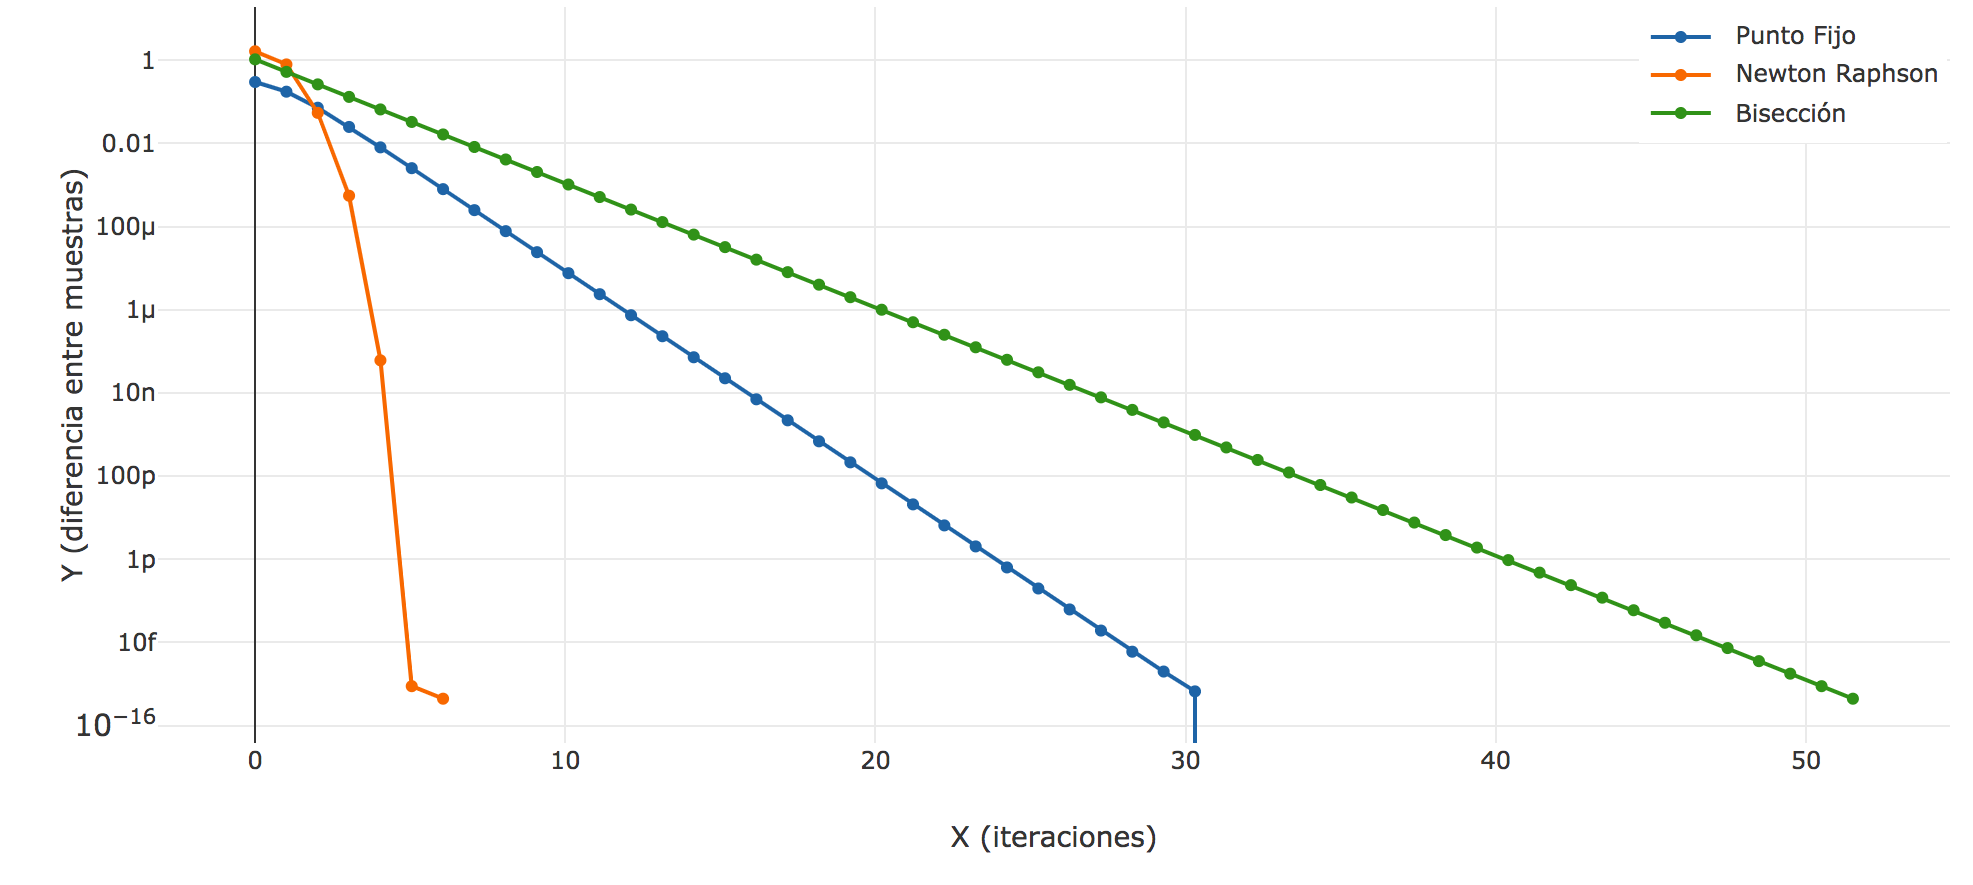
\includegraphics[width=15cm]{ej2-r1.png}
\end{centering}
\caption{Diferencias entre muestras para Raíz $X_{0}= -1.981$ por método.}
\end{figure}


$\mathbf{Raiz\; X_{1} =0.146 \pm0.5\;10^{-15}}$
\begin{figure}[H]
\begin{centering}
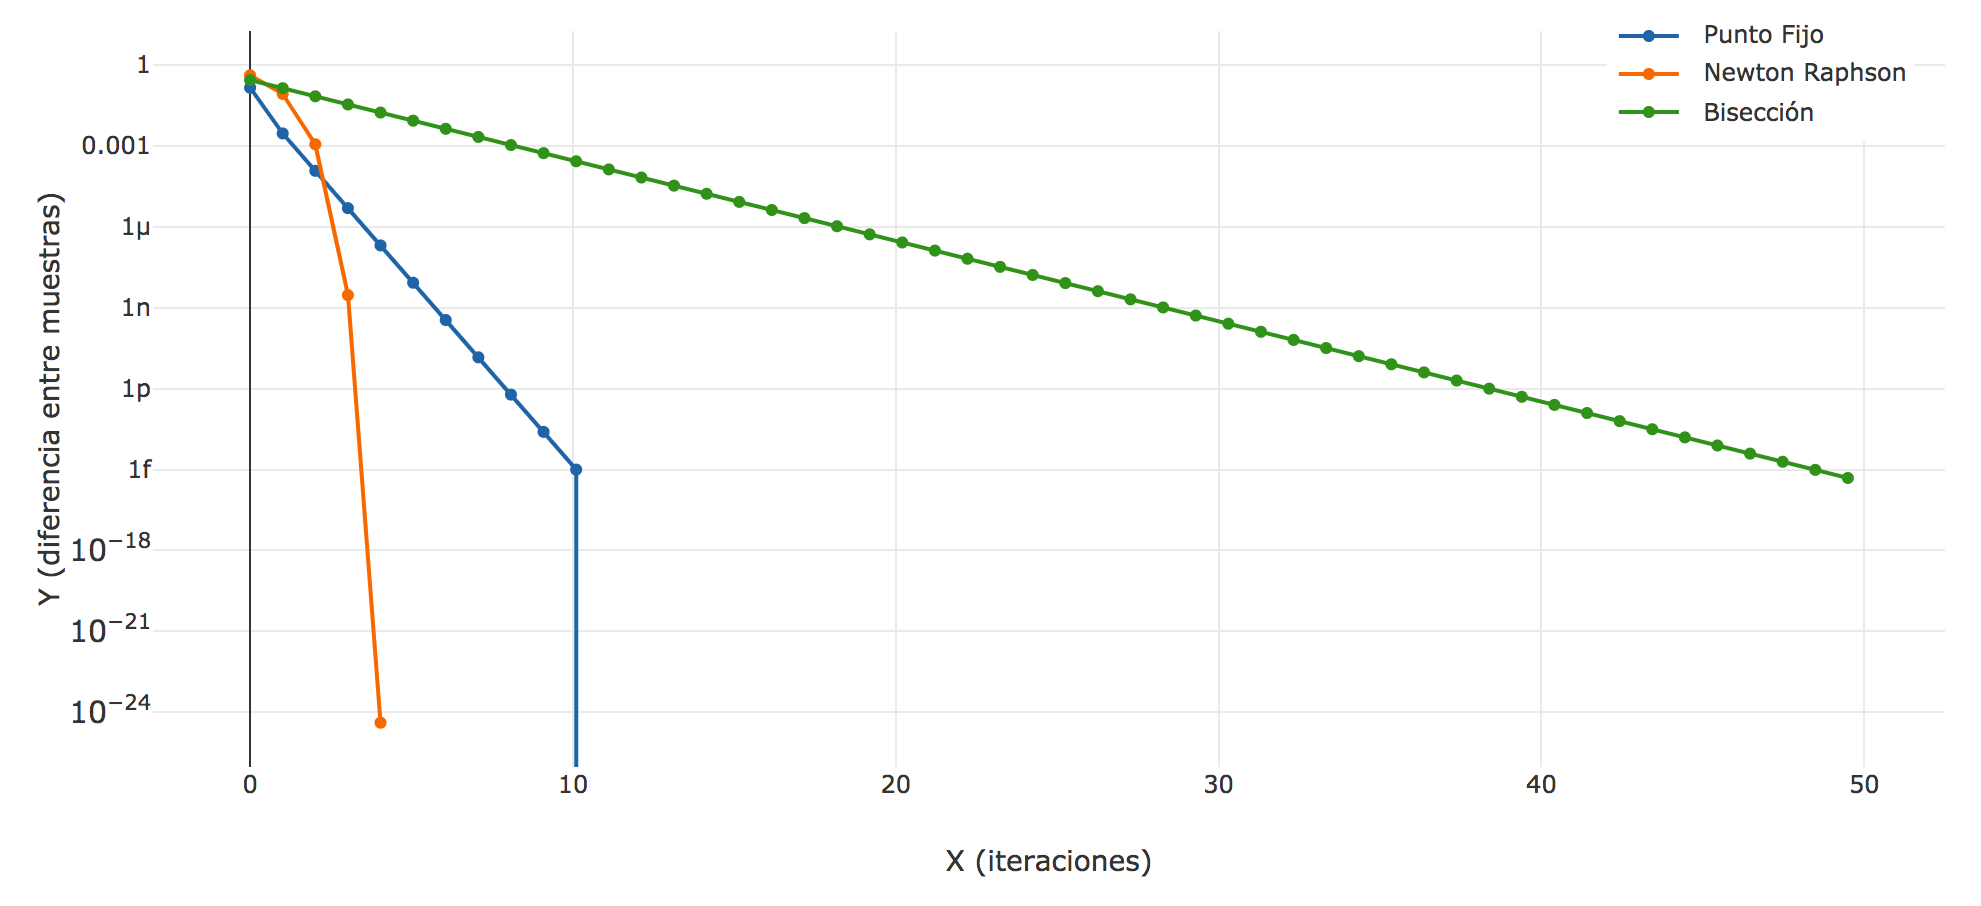
\includegraphics[width=15cm]{ej2-r2.png}
\end{centering}
\caption{Diferencias entre muestras para Raíz $X_{1}= 0.146$ por método.}
\end{figure}

$\mathbf{Raiz\; X_{2} = 1.583 \pm0.5\;10^{-15}}$
\begin{figure}[H]
\begin{centering}
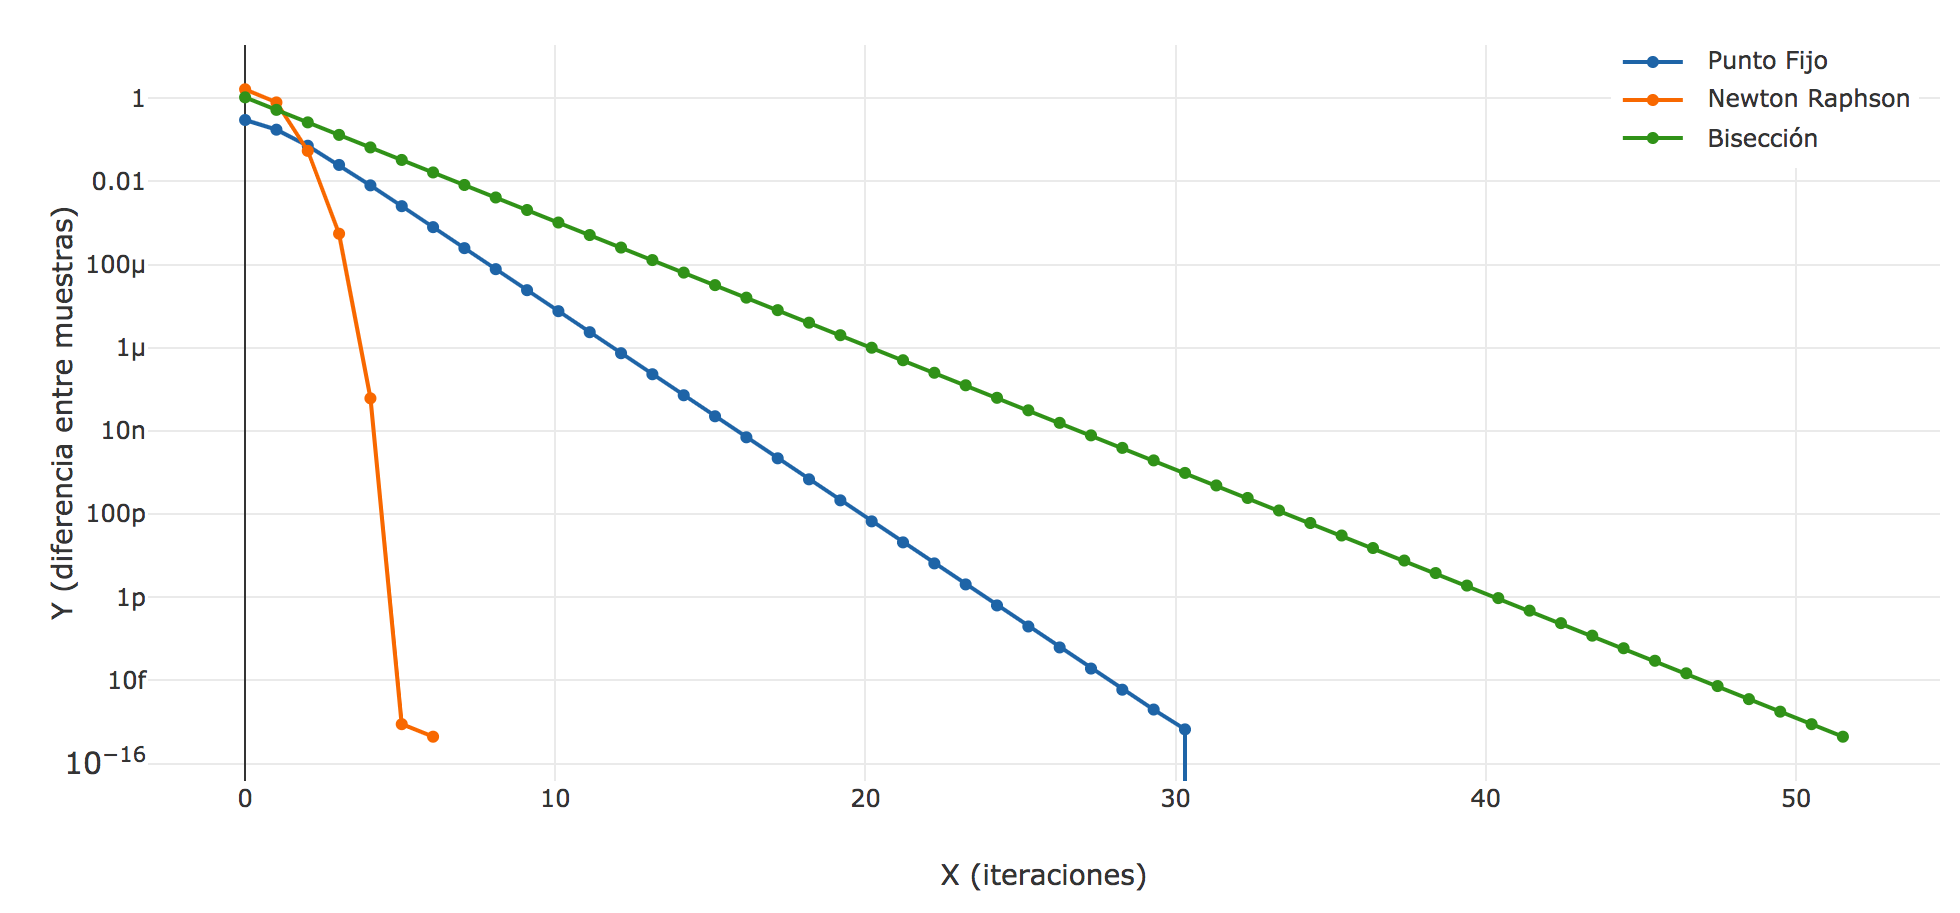
\includegraphics[width=15cm]{ej2-r3.png}
\end{centering}
\caption{Diferencias entre muestras para Raíz $X_{2} = 1.583$ por método.}
\end{figure}


\subsection{Ejercicio 3}
Para este punto, se busca encontrar el máximo intervalo de convergencia de cada raíz. Para esto, se desarrolló un algoritmo basado en el método de Newton-Raphson, de forma tal, que halle de manera secuencial los intervalos de convergencia de cada raíz. La función que implementa el algoritmo es intConv().\\

A partir de los cálculos del inciso 2, se conocen con una precisión apreciable, las tres raíces del sistema. Las usaremos para hallar los intervalos de convergencia.\\

\subsubsection{Algoritmo}

El algoritmo recibe la raíz $X_{i}$ y una precisión $\Delta x$ y se comporta de la siguiente manera

\begin{enumerate}[label=\roman*]
    \item La precisión pasada al algoritmo será $0,0001$ y 
    servirá de incremento a derecha y a izquierda de la raíz.\\
    \item Dentro de un ciclo, se hace desplazar al iterador incrementando $\Delta x$ a derecha de la raíz en cada turno.\\
    \item Se pregunta si Newton-Raphson de la posición $x_{0}+\Delta x$ converge a la raíz $X_{i}$.\\
    \item Se repite hasta que Newton-Raphson de la posición $x_{0}+\Delta x$ sea distinto de la raíz $X_{i}$ o la iteración supere los $\dfrac{50}{0.0001}=500000$ pasos (se mueva 50 unidades en el eje $x$).\\
    \item Si se superan las $50$ unidades en el eje $x$, el algoritmo tomará el extremo superior del intervalo como $+\infty$. \\
    \item El procedimiento es análogo para analizar el extremo inferior del intervalo (incrementando a izquierda).\\
\end{enumerate}

Para esta cantidad de iteraciones y de forma secuencial, el cálculo de los tres intervalos llevaba aproximadamente un minuto. Conociendo que la función tiene tres raíces, se puede evitar el cálculo del intervalo de convergencia para la raíz del medio. \\

Se acortó aproximadamente un tercio del tiempo de ejecución del cálculo de intervalos, mediante la inferencia del intervalo de convergencia de la raíz central.

\begin{equation}
\notag I(x_{0})=[x_{0}^{ini};x_{0}^{fin}]\hspace{30pt} I(x_{2})=[x_{2}^{ini};x_{2}^{fin}]\hspace{15pt}\Rightarrow \hspace{15pt} I(x_{1})=[x_{0}^{fin};x_{2}^{ini}]
\end{equation}

\subsubsection{Intervalos de Convergencia}
Para el método de Newton-Raphson fueron hallados los siguientes intervalos de convergencia con el algoritmo explicado anteriormente\\

\begin{itemize}
    \item Raíz $X_{0}=$ intervalo $[\infty\; ;\;-0.7838]$
    \item Raíz $X_{1}=$ intervalo $[-0.7837\;;\;0.7836]$
    \item Raíz $X_{2}=$ intervalo $[0.7837\;;\;\infty]$\\
\end{itemize}
 
\subsection{Ejercicio 4}

Para este ejercicio se necesita analizar el sistema variando el coeficiente que acompaña a la masa $m_0$. No hace falta volver a calcular la derivada de la función $F_{Res}$ ya que el término que depende de la masa $m$, no depende de la variable $y$.\\

Para conocer la estabilidad o inestabilidad de los puntos de equilibrio de $F_{Res}$, se deberá calcular la segunda derivada de la energía potencial $U$ del sistema y luego, analizar su signo en cada raíz $X_{i}$\\

%Evaluando esta expresión en las raicopuesto de la derivada de la función y ver el signo de $\dfrac{d\;F_{Res}(X_{i})}{dy}$. 

Recordando que $\dfrac{dU}{dy}=-\sum{F_{Cons}} (y)$ es posible hallar fácilmente la expresión $\dfrac{d^{2}U}{dy^{2}}$ derivando  $-F_{Res}$\\

\begin{itemize}
    \item Si $-\dfrac{d\;F_{Res}(X_{i})}{dy} < 0 $ es un punto de equilibrio inestable.
    \item Si $-\dfrac{d\;F_{Res}(X_{i})}{dy} = 0 $ es un punto de equilibrio indiferente o neutral.
    \item Si $-\dfrac{d\;F_{Res}(X_{i})}{dy} > 0 $ es un punto de equilibrio estable.
\end{itemize}

Usando la expresión despejada anteriormente se puede saber que \\

\begin{equation}
\begin{aligned}
\notag - f'(y)&=2k+\dfrac{2kL_{0}y^{2}}{(1 + y^{2})^{3/2}} - \dfrac{2kL_{0}}{\sqrt{1 + y^{2}}}\\[10pt]
- f'(y)&=20+\dfrac{41.02\;.\;y^{2}}{(1 + y^{2})^{3/2}} - \dfrac{41.02}{\sqrt{1 + y^{2}}}
 \end{aligned}
\end{equation}\\

Haciendo los cálculos para hallar el tipo de equilibrio para cada caso\\

\begin{table}[H]
\makegapedcells
\centering
\resizebox{0.7\textwidth}{!}{
\begin{tabular}{|c|c|c|c|c|c|c|}
\hline            & $-F'_{Res}(X_{0})$ & $-F'_{Res}(X_{1})$ & $-F'_{Res}(X_{2})$  \\
\hline $0$        & $-F'(-1.79)=15.23$ & $-F'(0)=-21.02$ & $-F'(1.79)=15.23$\\
\hline $0,3m_{0}$ & $ -F'(-1.98)=16.24$ & $-F'(0.14)=-19.84$ &$ -F'( 1.58)=13.72$ \\
\hline $0,6m_{0}$ &$ -F'(-2.16)=16.96$ & $-F'(0.32)=-15.43$ & $-F'(1.34)=11.22$ \\
\hline $0,9m_{0}$ &  $-F'(-2.33)=17.51$ & $-F'(0.59)=-6.21$ & $-F'(0.99)=5.27$\\
\hline $1,2m_{0}$ & $-F'(-2.51)=17.92$ &$\nexists$&$\nexists$ \\
\hline $1,5m_{0}$ & $-F'(-2.68)=18.24$ &$\nexists$&$\nexists$ \\
\hline
\end{tabular}}
\end{table}


\subsubsection{Tabla Comparativa de distintos métodos}

\begin{table}[H]
\makegapedcells
\centering
\resizebox{1\textwidth}{!}{
\begin{tabular}{|c|c|c|c|c|c|c|}
\hline            & $X_{0}$ & Equilibrio & $X_{1}$ & Equilibrio & $X_{2}$ & Equilibrio \\
\hline $0$        & -1.790698467079257 &  Estable  & 0.000000000000000 & Inestable  & 1.7906984670792565 & Estable    \\
\hline $0,3m_{0}$ & -1.981951862586309 & Estable & 0.146531069947676 & Inestable & 1.583239767691588 & Estable \\
\hline $0,6m_{0}$ & -2.163386121522913 & Estable & 0.315566691472281 & Inestable & 1.343701800526605 & Estable \\
\hline $0,9m_{0}$ & -2.338269945230656 & Estable & 0.590881634987573 & Inestable & 0.991825978297377 &  Estable \\
\hline $1,2m_{0}$ & -2.508510978388360 & Estable & $\nexists$ &- & $\nexists$ & - \\
\hline $1,5m_{0}$ & -2.675319915043171 & Estable & $\nexists$ & - & $\nexists$ & - \\
\hline
\end{tabular}}
\end{table}


\section{Conclusiones}

Se consiguió calcular de manera satisfactoria los puntos de equilibrio del sistema de dos resortes con una masa despejando de forma numérica a través de distintos métodos.

De parte del equipo, nos ha parecido muy interesante la posibilidad de efectuar cálculos sin la necesidad de tener los valores resultantes de la función de forma analítica.




%----------------------------------------------------------------------------------------
%	BIBLIOGRAPHY
%----------------------------------------------------------------------------------------

%\bibliographystyle{apalike}
%\bibliography{sample}
%----------------------------------------------------------------------------------------


\end{document}
